\chapter{Force-Aware Imitation Learning for Local Difficult Regions}
\label{chap:force_il}
\section{Motivation and Scope}
The local policy is designed for short segments that are difficult to cover reliably with a single global geometric strategy. Representative regions include body edges, cutaways, neck joints, fret areas, pickup covers, bridges, and narrow hardware clearances. The method is not intended to replace the CAD planner on broad surfaces, where explicit coverage and removal objectives are easier to verify.

Imitation learning is selected instead of unrestricted RL because a skilled operator can directly demonstrate the required approach direction, tool tilt, force reduction, repeated stroke, and termination. Real-world trial-and-error is expensive and potentially destructive, and a complete local-finishing reward would require difficult weighting among coverage, collision, force, surface damage, and stopping.

\begin{figure}[t]
    \centering
    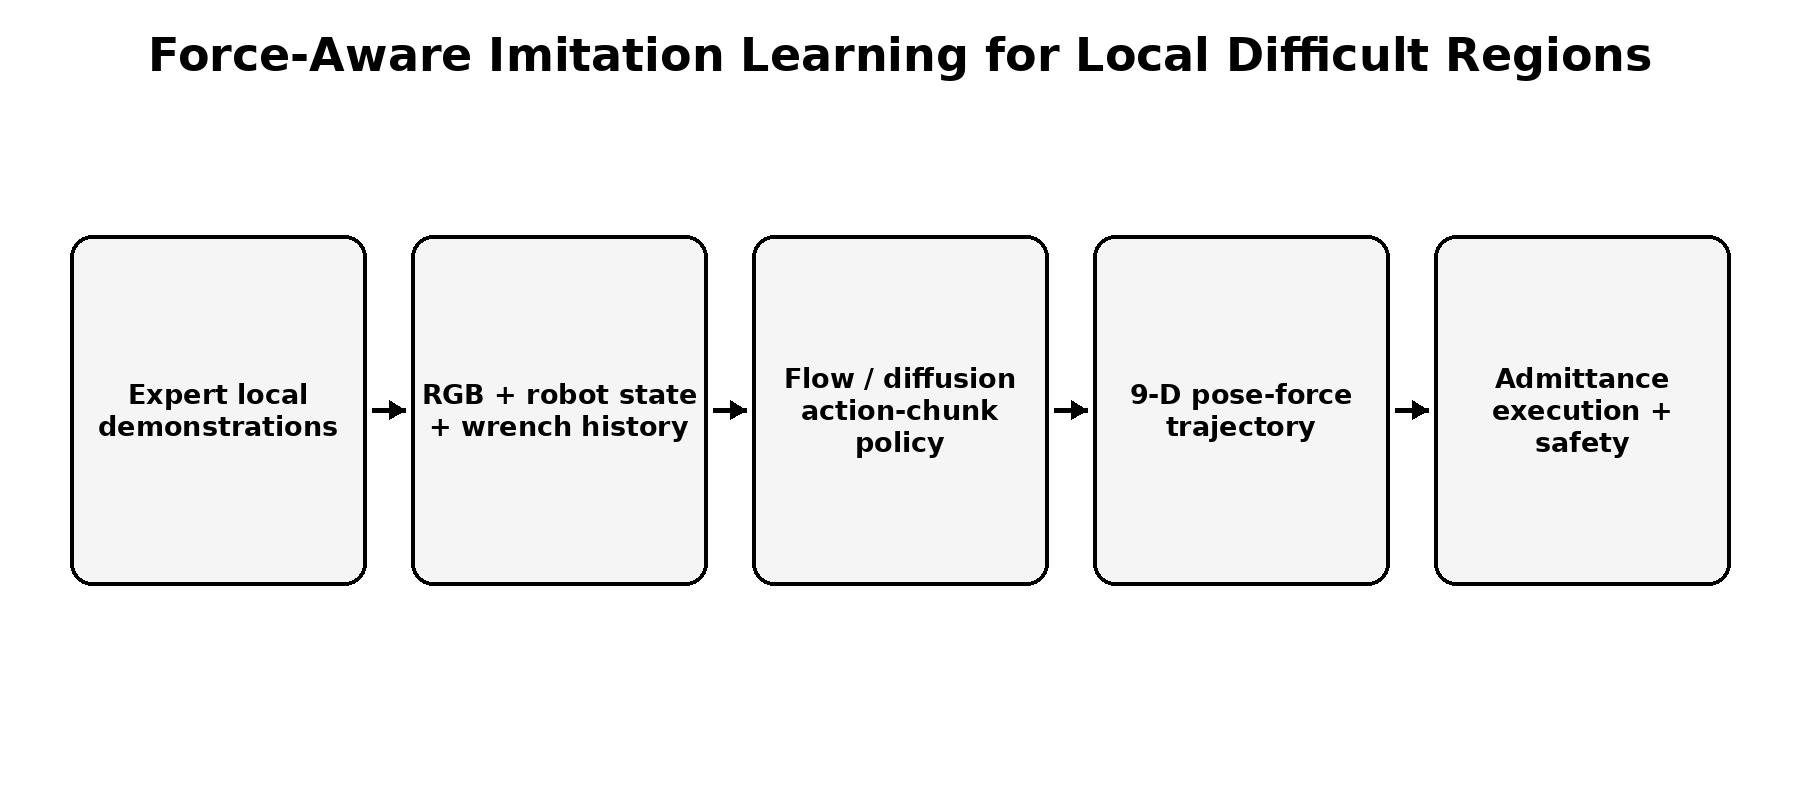
\includegraphics[width=0.98\textwidth]{./5.ForceAwareIL/figs/force_aware_il_pipeline.png}
    \caption{Force-aware imitation-learning pipeline for local difficult regions.}
    \label{fig:force_il_pipeline}
\end{figure}

\section{Demonstration Data}
Each demonstration contains synchronized local RGB observations, optional masks, robot or demonstrator pose, six-axis wrench, spindle state, region identity, and termination labels. Demonstrations can be collected through force-feedback teleoperation, kinesthetic teaching with a passive tool, or a force-motion capture device. The dataset is segmented into approach, contact, processing, and retraction phases.

Force signals are bias-corrected, transformed to the tool frame, and filtered without eliminating contact onset or impact transients. Failed demonstrations are rejected or labeled explicitly. The local nature of the task reduces the duration and quantity of demonstrations compared with teaching the entire product surface.

\section{Observation and Action}
Before the feature-masking extension of Chapter~\ref{chap:feature_masking}, the baseline observation is
\begin{equation}
\mathbf{o}_t^{\mathrm{IL}}=\{I_t,\mathbf{s}_t,\mathbf{H}_{t}^{w}\},
\end{equation}
where $I_t$ is the RGB image, $\mathbf{s}_t$ is the robot state, and $\mathbf{H}_{t}^{w}$ is the recent wrench history. The action is an $H$-step chunk of 9-D pose--force waypoints:
\begin{equation}
\mathbf{A}_t=[\mathbf{a}_t,\mathbf{a}_{t+1},\ldots,\mathbf{a}_{t+H-1}]\in\mathbb{R}^{H\times9}.
\end{equation}
Only the first part of the chunk is executed before the policy replans from the latest observation.

\section{Policy Architecture}
A visual encoder extracts image features, a temporal encoder processes the wrench history, and a state encoder processes pose and velocity. The modalities are fused and passed to a conditional flow-matching or diffusion action generator. A generative action-chunk policy is preferred over one-step regression because multiple safe local trajectories may exist around the same hardware geometry.

\section{Direct Desired-Force Generation}
The policy explicitly predicts the desired Cartesian force together with motion. This differs from force-as-observation-only policies and from methods that convert force into a virtual positional target. Nevertheless, ForceMimic predicts wrench-position parameters and executes them using hybrid force-position control~\cite{liu2025forcemimic}, while Min et al. separate desired motion and desired force for complex wooden-surface finishing~\cite{min2024force}. The thesis therefore treats direct force output as one component of the contribution, not as the complete novelty claim.

\section{Low-Level Execution and Safety}
The desired pose--force chunk is passed to the common admittance controller. The safety supervisor validates workspace, collision margin, force, torque, velocity, spindle state, and cumulative dwell. Out-of-distribution detection can use latent feature distance, ensemble disagreement, or a task-specific confidence model. Low confidence triggers a stop or operator request rather than autonomous extrapolation.

\section{Baselines and Ablations}
The local policy is compared with a manually programmed path, RGB-only IL with fixed force, RGB-plus-wrench IL with fixed force, and direct 9-D pose--force IL. Ablations include wrench history length, action horizon, force observation, direct force output, flow matching versus deterministic behavior cloning, and task-relevant masking.
